%%%%%%%%%%%%%%%%%%%%%%%%%%%%%%%%%%%%%%%%%
% Arsclassica Article
% LaTeX Template
% Version 1.0 (21/4/14)
%
% Original author:
% Lorenzo Pantieri (http://www.lorenzopantieri.net) with extensive modifications by:
% Vel (vel@latextemplates.com)
%
% License:
% CC BY-NC-SA 3.0 (http://creativecommons.org/licenses/by-nc-sa/3.0/)
%%%%%%%%%%%%%%%%%%%%%%%%%%%%%%%%%%%%%%%%%

%----------------------------------------------------------------------------------------
%	PACKAGES AND OTHER DOCUMENT CONFIGURATIONS
%----------------------------------------------------------------------------------------

\documentclass[
10pt, % Main document font size
a4paper,
oneside, % One page layout (no page indentation)
%twoside, % Two page layout (page indentation for binding and different headers)
headinclude,footinclude, % Extra spacing for the header and footer
BCOR5mm, % Binding correction
]{scrreprt}

%%%%%%%%%%%%%%%%%%%%%%%%%%%%%%%%%%%%%%%%%
% Arsclassica Article
% Structure Specification File
%
% Original author:
% Lorenzo Pantieri (http://www.lorenzopantieri.net) with extensive modifications by:
% Vel (vel@latextemplates.com)
%
% License:
% CC BY-NC-SA 3.0 (http://creativecommons.org/licenses/by-nc-sa/3.0/)
%%%%%%%%%%%%%%%%%%%%%%%%%%%%%%%%%%%%%%%%%

%----------------------------------------------------------------------------------------
%	REQUIRED PACKAGES
%----------------------------------------------------------------------------------------
\usepackage[
nochapters, % Turn off chapters since this is an article        
beramono, % Use the Bera Mono font for monospaced text (\texttt)
eulermath,% Use the Euler font for mathematics
pdfspacing, % Makes use of pdftex’ letter spacing capabilities via the microtype package
dottedtoc % Dotted lines leading to the page numbers in the table of contents
]{classicthesis} % The layout is based on the Classic Thesis style

\usepackage{arsclassica} % Modifies the Classic Thesis package

\usepackage[french]{babel}

\usepackage[T1]{fontenc} % Use 8-bit encoding that has 256 glyphs

\usepackage[utf8]{inputenc} % Required for including letters with accents

\usepackage{graphicx} % Required for including images

\graphicspath{{figures/}} % Set the default folder for images

\usepackage{enumitem} % Required for manipulating the whitespace between and within lists

\usepackage{lipsum} % Used for inserting dummy 'Lorem ipsum' text into the template

%\usepackage{subfig} % Required for creating figures with multiple parts (subfigures)

\usepackage{amsmath,amssymb,amsthm} % For including math equations, theorems, symbols, etc

\usepackage[french]{varioref} % More descriptive referencing

\usepackage{verbatimbox} % Centered verbatim

\usepackage{caption}

\usepackage{subcaption}
\usepackage{algorithm2e}
%----------------------------------------------------------------------------------------
%	THEOREM STYLES
%---------------------------------------------------------------------------------------
\theoremstyle{definition} % Define theorem styles here based on the definition style (used for definitions and examples)
\newtheorem{definition}{Definition}

\theoremstyle{plain} % Define theorem styles here based on the plain style (used for theorems, lemmas, propositions)
\newtheorem{theorem}{Theorem}

\theoremstyle{remark} % Define theorem styles here based on the remark style (used for remarks and notes)

%----------------------------------------------------------------------------------------
%	HYPERLINKS
%---------------------------------------------------------------------------------------
\hypersetup{
%draft, % Uncomment to remove all links (useful for printing in black and white)
colorlinks=true, breaklinks=true, bookmarks=true,bookmarksnumbered,
urlcolor=webbrown, linkcolor=RoyalBlue, citecolor=webgreen, % Link colors
pdftitle={}, % PDF title
pdfauthor={\textcopyright}, % PDF Author
pdfsubject={}, % PDF Subject
pdfkeywords={}, % PDF Keywords
pdfcreator={pdfLaTeX}, % PDF Creator
pdfproducer={LaTeX with hyperref and ClassicThesis} % PDF producer
} % Include the structure.tex

\hyphenation{Fortran hy-phen-ation}

%----------------------------------------------------------------------------------------
%	TITLE AND AUTHOR(S)
%----------------------------------------------------------------------------------------
\title{Flow}
\title{\normalfont\spacedallcaps{Flow}}

\date{}

%----------------------------------------------------------------------------------------

\begin{document}

%----------------------------------------------------------------------------------------
%	HEADERS
%----------------------------------------------------------------------------------------

\renewcommand{\sectionmark}[1]{\markright{\spacedlowsmallcaps{#1}}} % The header for all pages
%\renewcommand{\subsectionmark}[1]{\markright{\thesubsection~#1}} % this modifies the header on odd pages
\lehead{\mbox{\llap{\small\thepage\kern1em\color{halfgray} \vline}\color{halfgray}\hspace{0.5em}\rightmark\hfil}}

\pagestyle{scrheadings}

%----------------------------------------------------------------------------------------
%	TABLE OF CONTENTS & LISTS OF FIGURES AND TABLES
%----------------------------------------------------------------------------------------

\date{Revision to consider : 73}

\maketitle

\setcounter{tocdepth}{2}

\tableofcontents

\listoffigures

%\listoftables

\newpage

%----------------------------------------------------------------------------------------
%	INTRODUCTION
%----------------------------------------------------------------------------------------
\section*{Introduction}
Flow est originellement un jeu de reflexion. Le principe consiste à remplir une grille dans sa totalité en reliant les points de même couleur.

On comprend déjà que notre algorithme de résolution va chercher à trouver des parcours qui vont à la fois chercher à relier les couleurs correspondantes et couvrir le plus d'espace possible sans se géner entre eux.

Nous allons donc poser dans un premier temps les problèmes à résoudre ainsi que le vocabulaire que nous allons employer pour caractériser le jeu. Nous verrons ensuite comment nous avons implémenté les types abstraits de données qui apparaissent dans les problèmes évoqués ci-dessus puis nous terminerons par présenter l'algorithme de résolution et l'ensemble des tests réalisés pour vérifier sa validité.

\subsection*{Capacité du programme réalisé}

Notre programme permet d'afficher, de jouer et de résoudre une grille carrée donnée en paramètre.
La résolution ne gère pas les grilles comportant des ponts.
Le programme résout des grilles de taille variable (mais carrées). Il n'y a pas de limite ormis que le programme prendra plus de temps pour des grilles de grande taille.

Le résolution ne vérifie pas si toutes les cases sont coloriées. Par conséquent, le programme propose parfois en résolution, une grille ou tous les chemins rejoignent bien les cases de même couleur mais où certaines cases sont vides.

%----------------------------------------------------------------------------------------

\newpage

%----------------------------------------------------------------------------------------
%	ALGORITHMIQUE DU JEU
%----------------------------------------------------------------------------------------
\chapter{Algorithmique du jeu}

%----------------------------------------------------------------------------------------
%	DÉFINITIONS
%----------------------------------------------------------------------------------------
\section{Définitions}
Les mots que nous allons utiliser pour décrire un objet ou un concept précis mis en oeuvre dans la résolution du problème sont des mots pouvant donner lieu à de nombreuses lectures et approches différentes qui peuvent fausser les démonstrations qui s'appuient dessus. Pour fixer les idées, nous nous devons d'imposer des bases, seul appui pour nos raisonnements ultérieurs.

\label{sect:def}
Une \textit{case} $c$ sera considéré comme une élément admettant une unique couleur (que l'on pourra étiqueter par un entier positif) dans l'ensemble $\Omega$. On admettra pour simplifier que 0 correspond à une abscence de couleur (on dira que la case n'est pas coloriée) et on pourra assimiler cet ensemble à $\mathbb{R}_+$.

Une \textit{grille} $\mathcal{G}$ est une matrice de cases, à laquelle est associée une fonction $\eta_\mathcal{G} : C\rightarrow \Omega$, où $C$ est l'ensemble des cases de la grille et $\forall c\in C, \exists \omega\in \Omega : \eta_\mathcal{G}(c) = \omega$, où $\omega$ est la couleur de la case $c$.

Une case \textit{primaire} est une case qui possède une couleur fixée dans la grille \textit{vide} correspondant à $\mathcal{G}$.

Une case sera dite \textit{remplie} si son état est dans $\Omega^*$.

On définie la notion de \textit{chemin de couleur $\omega$} comme étant une succession de cases de couleur $\omega$ de la grille formant un ensemble 4-connexe. De fait, deux chemins sur la grille ne peuvent pas s'intersecter. Un chemin est \textit{valide} s'il débute dans une case primaire et aboutit dans une autre case primaire.

On appelle cases \textit{adjacentes} deux cases liées par une arrête et qui partagent une couleur commune (deux cases successives sur un chemin associé à une couleur).

%----------------------------------------------------------------------------------------
%	PROBLÈMES
%----------------------------------------------------------------------------------------
\section{Problèmes}
\subsection{Présentation du jeu}
Le jeu Flow consiste à déterminer les chemins valides de chaque couleur dans la grille, et idéalement, à fixer la couleur de chacune des cases. Pour cela, nous devons passer par des étapes de lecture d'une fichier de grille, puis de résolution et enfin d'affichage. Dans cette partie, nous chercherons à présenter les algorithmes principaux utilisées.

\subsection{Spécifications}
Le premier problème auquel nous pouvons nous intéresser est un problème de validation d'une grille remplie (après que l'utilisateur ait joué au jeu par exemple). Le problème est spécifié de la façon suivante :

\begin{verbatim}
Problème : Validation
Entrée : Une grille G remplie.
Sortie : Un booléen indiquant si la grille est valide ou non.
\end{verbatim}

Pour la résolution de ce problème, on doit vérifier les points suivants :
\begin{itemize}
\item pour chaque couleur, l'ensemble des cases de cette couleur doit être connexe,
\item les cases d'une même couleur forment un chemin sans boucles,
\item ce chemin débute dans une case primaire pour aboutir dans une autre case primaire.
\end{itemize}

Comme à chaque case est associée une unique couleur, on interdit ici toute intersection non-vide entre les ensemble de différentes couleurs.

Le second problème que nous avons traité est le problème d'existence ou non d'une solution, spécifié de la façon suivante :

\begin{verbatim}
Problème : Resolution
Entrée : Une grille G.
Sortie : Une grille R et un booléen r tel que :
    r = FAUX s'il n'existe pas de solutions de G,
    r = VRAI si R est une solution de G.
\end{verbatim}

\subsection{Algorithmes}
\subsubsection{Validation}
La fonction principale du moteur de jeu est la vérification d'une grille résolue. En effet le moteur graphique gère la jouablilité d'un coup, ce qui enlève des possibilités de coups et réduit la complexité de la vérification. \\

	Par exemple, une grille où des sommets colorés non primaires non relié à des sommets primaires n'est pas une grille que nous pouvons obtenir avec notre moteur graphique. \\

L'algorithme fonctionne de la façon suivante : \\
\begin{algorithm}[H]
 \KwData{Graphe représentant la grille}
 \KwResult{Booléen Vrai si la grille est bien remplie, Faux sinon}
 
 \While{Toutes les couleurs n'ont pas été testées}{
  Choisir nouvelle couleur\;
  Chercher sommet primaire correspondant\;
  Stocker l'indice de ce sommet\;
  	\While{Sommet courant n'est pas primaire de clé différente de celle stockée}{
		\eIf{Sommet courant est primaire de même clé}{
				retourner Faux\;
		}	
		{
				Passer au sommet voisin\;
		}

	}
		
  retourner Vrai\;
}
\caption{Vérification de grille}
\end{algorithm}

	Dans notre implémentation, le degré de chaque sommet est limité à deux. Lorsque deux sommets sont adjacents sur la grille, de la même couleur mais non liés, le parcours se fera correctement.\\
    
    De plus, chaque sommet coloré étant lié à un sommet primaire, les seuls cas où l'algorithme retournera faux sont lorsque la grille n'est pas complétement remplie, ou lorsque qu'un chemin n'atteint pas un sommet primaire distinct. Nos listes d'adjacences se remplissent en tête, lorsqu'un sommet est au bout d'un chemin, il n'a qu'un seul voisin. En fait, l'algorithme retournera en arrière et parcourera le même chemin une seconde fois. Il se stoppera en arrivant sur un sommet primaire de même clé que celui de départ.

L'algorithme de validation a été construit avec l'interface graphique utilisant la librairie \textit{ltk}. L'utilisateur lorsqu'il joue au jeu ne peux pas effectuer certaines actions, comme relier deux cases de couleurs différentes, intersecter des chemins, etc. Par conséquent, la difficulté de notre fonction de validation se retrouve transférée à la gestion de l'interface graphique elle-même, et nous avons ainsi une fonction de valisation qui n'effectue que des vérifications de base pour valider un remplissage.

\subsubsection{Résolution}
Notre algorithme de résolution s'inspire de la recherche en profondeur dans un graphe (DFS). Son principe consiste à construire récursivement les chemins reliant les couleurs de la grille en appelant à chaque étape une recherche en profondeur qui tient compte des modifications apportés.

Considérons la grille de jeu représentée sur la Figure~\vref{subfig:start}. Avant de décrire le déroulement de l'algorithme sur cette grille nous allons mettre au point un certain nombre de conventions utiles pour la suite. Premièrement, à chaque couleur nous attribuons les entiers suivants (Rouge:1, Orange:2, Jaune:3, Bleu:4, Vert:5).

Deuxièmement, si l'algorithme est amené à choisir une direction où se déplacer, il devra la choisir selon l'ordre suivant : nord, est, sud, ouest. Ces conventions sont totalement arbitraires, néanmoins elles servent à prendre des décisions pendant l'éxéution des instructions. Finalement, nous appellerons obstacle les bords de la grille ou un noeud de couleur différentes de la couleur recherchée.\\

A l'état initial, le solver choisit la première couleur à relier, celle correspondant à l'entier le plus faible (Rouge). Ensuite, il en détermine une position dans la grille et choisit une direction disponible pour se déplacer (nord). Puis, il se déplace en ligne droite  suivant cette direction jusqu'à rencontrer un obstacle (bords de la grille) (cf. Figure~\vref{subfig:p1}).

Arrivé à cet étape, le solver doit encore décider d'une direction vers laquelle il va tourner (est) (cf. Figure~\vref{subfig:p2}). Si aucune direction n'est disponible, le solver retourne en arrière d'une case jusqu'à en trouver une. Ce processus est répeté jusqu'à ce que le solver tombe sur un noeud primaire ayant la même couleur à relier et différent du noeud de départ. Les Figures~\vref{subfig:p4} et ~\vref{subfig:p3} correspondent à des états intermédiares, on y voit notamment le solveur changer de direction lorsqu'il ne trouve aucune issue. La Figue ~\vref{subfig:p5} correspond à la fin de la recherche pour la couleur rouge.

La prochaine étape va consister à relier la deuxième couleur d'entier le plus faible (Orange). Toujours en suivant les même règles de recherche, nous constatons qu'au bout de quelques déplacements le chemin rouge bloque le chemin orange (cf. Figure~\vref{subfig:p6}), le solveur fait donc des retours en arrière, ce qui le conduit en fin de compte à retracer un nouveau chemin pour la couleur rouge (cf. Figure~\vref{subfig:p7}). Cette fois-çi la voie est libre pour le chemin orange qui peut se déplacer vers l'est (cf. Figure~\vref{subfig:p8}). Le solveur va continuer ainsi à appliquer les mêmes règles jusqu'à relier toutes les couleurs dans l'ordre croissant des entiers qui leurs sont attribués (cf. Figure~\vref{subfig:p9}).\\

A partir de cette description, nous pouvons constater que l'algorithme est amené à plusieurs reprises à prendre des décisions influancant ses déplacements. Ses décisions concernent notamment, le choix de la couleur, le choix de la direction, le déplacement en ligne droite et le retour en arrière. L'algorithme doit aussi identifier quelques situations particulières : aucun déplacement possible, obstacle atteint, couleur reliée.

\begin{figure}[h]
  \centering
  \begin{subfigure}[b]{0.3\textwidth}
      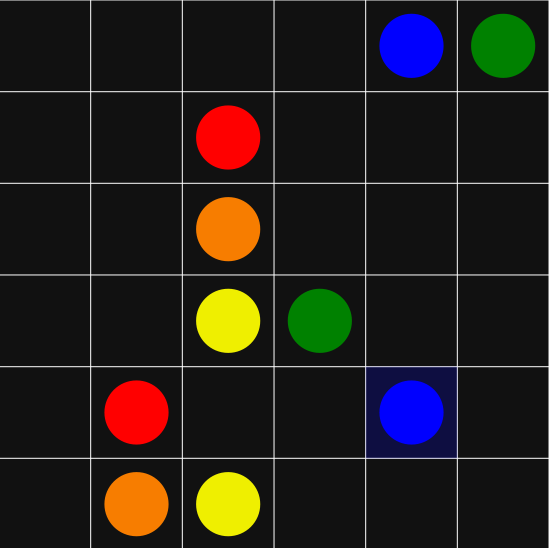
\includegraphics[width=\linewidth]{start.png}
      \caption{Grille de départ}
      \label{subfig:start}
   \end{subfigure}
   \begin{subfigure}[b]{0.3\textwidth}
      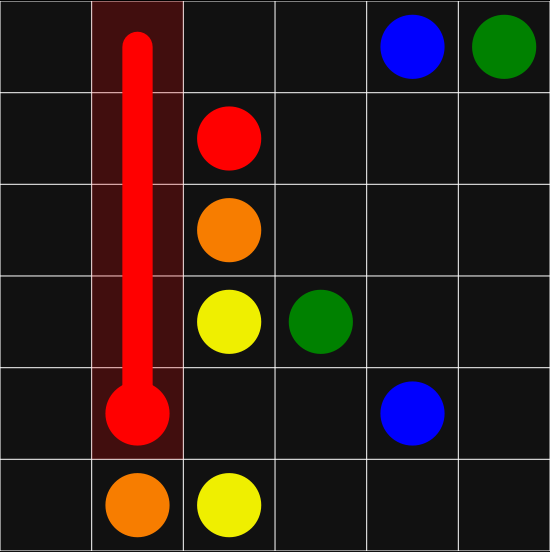
\includegraphics[width=\linewidth]{p1.png}
      \caption{Obstacle trouvé}
      \label{subfig:p1}
   \end{subfigure}
   \begin{subfigure}[b]{0.3\textwidth}
      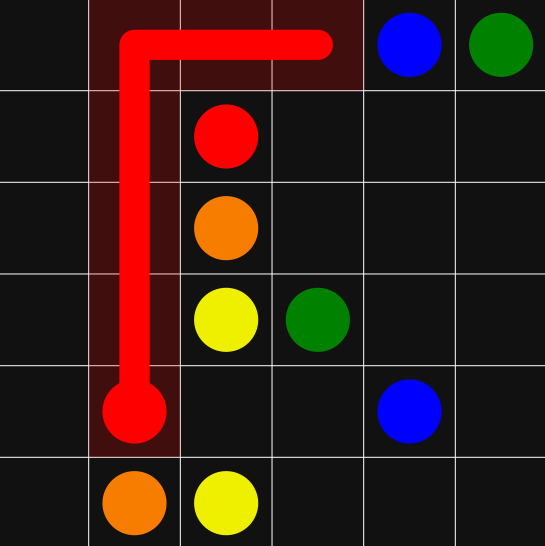
\includegraphics[width=\linewidth]{p2.png}
      \caption{Aller vers l'Est}
      \label{subfig:p2}
   \end{subfigure}
   \begin{subfigure}[b]{0.3\textwidth}
      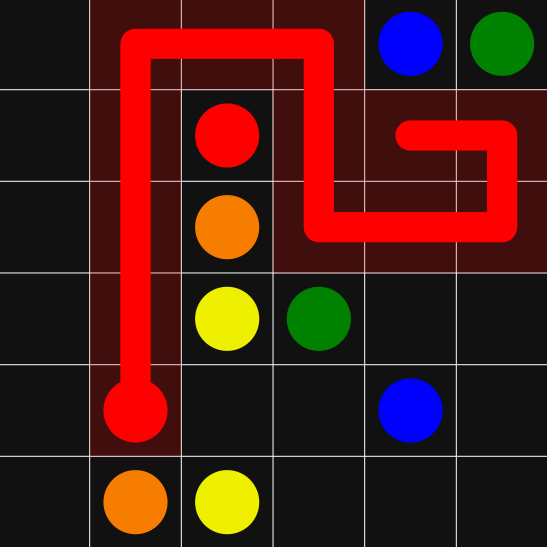
\includegraphics[width=\linewidth]{p4.png}
      \caption{Aucune issue}
      \label{subfig:p4}
   \end{subfigure}
   \begin{subfigure}[b]{0.3\textwidth}
      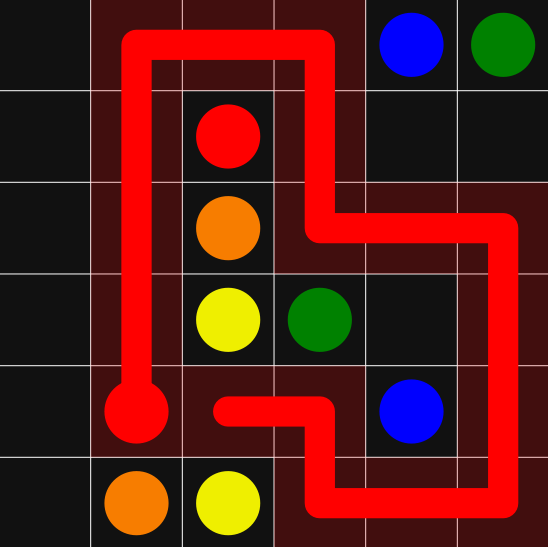
\includegraphics[width=\linewidth]{p3.png}
      \caption{Aucune issue}
      \label{subfig:p3}
   \end{subfigure}
   \begin{subfigure}[b]{0.3\textwidth}
      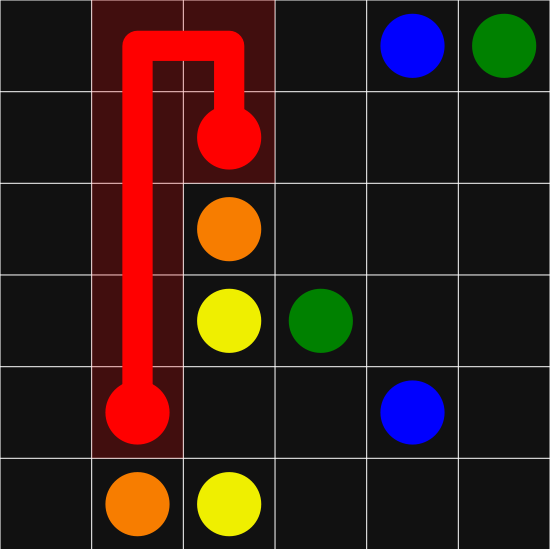
\includegraphics[width=\linewidth]{p5.png}
      \caption{Couleur reliée}
      \label{subfig:p5}
   \end{subfigure}
   \begin{subfigure}[b]{0.3\textwidth}
      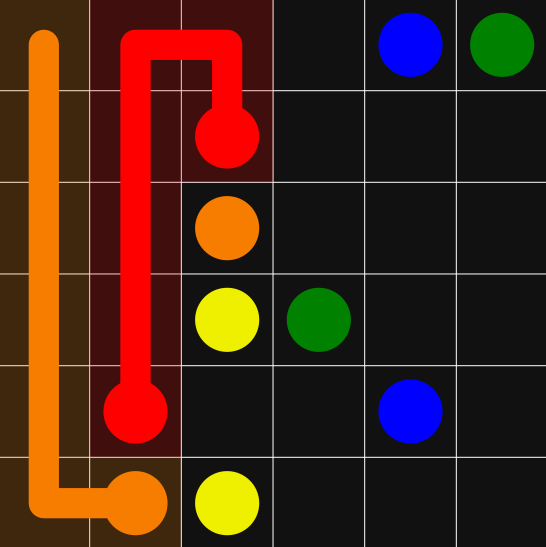
\includegraphics[width=\linewidth]{p6.png}
      \caption{Orange bloqué}
      \label{subfig:p6}
   \end{subfigure}
   \begin{subfigure}[b]{0.3\textwidth}
      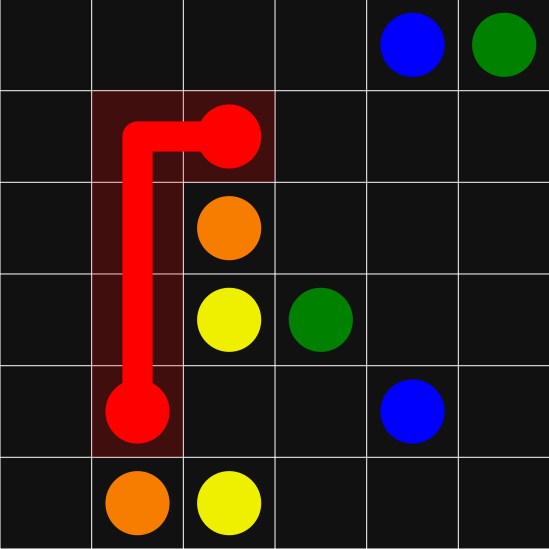
\includegraphics[width=\linewidth]{p7.png}
      \caption{Rouge rectifié}
      \label{subfig:p7}
   \end{subfigure}
   \begin{subfigure}[b]{0.3\textwidth}
      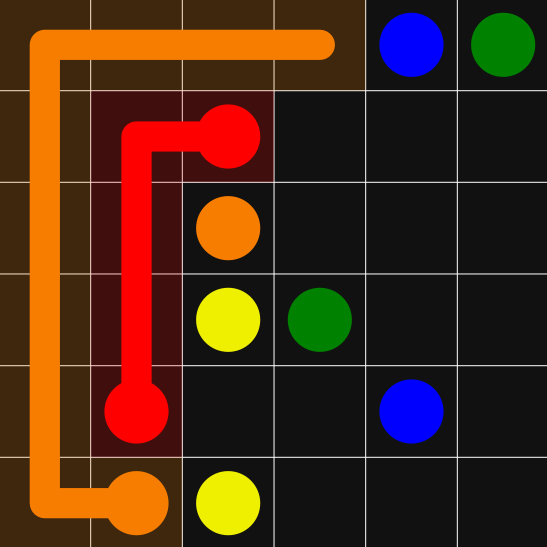
\includegraphics[width=\linewidth]{p8.png}
      \caption{Orange libre}
      \label{subfig:p8}
   \end{subfigure}
   \begin{subfigure}[b]{0.3\textwidth}
      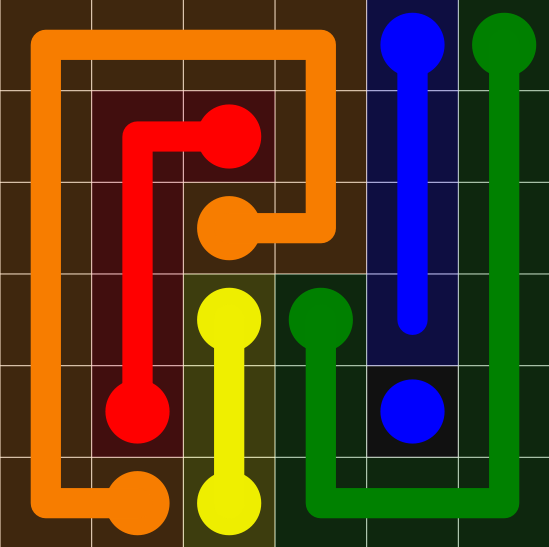
\includegraphics[width=\linewidth]{p9.png}
      \caption{Dernière étape}
      \label{subfig:p9}
   \end{subfigure}
   \label{fig:etapes}
   \caption{Étapes de résolution}
\end{figure}



%---------------------------------------------------------------------------
%   REALISATION
%---------------------------------------------------------------------------
\chapter{Réalisation du Programme}
\section{Structure des données}
\subsection{Structure grille}

La grille fournie en entrée est un fichier texte contenant les dimensions de la grille ainsi qu'une matrice symbolisant la grille tel que:
\begin{itemize}
	\item Un \# signifie une case vide.
    \item Un entier de signifie une case colorée primaire.
    \item Un + signifie un pont.
\end{itemize}

\begin{verbbox}
4 4
#1#3
#3#2
1#+#
2#44
\end{verbbox}
\begin{figure}[ht]
	\centering
	\theverbbox
	\caption{Exemple de grille $4\times 4$}
	\label{fig:ex_grille}
\end{figure}

Pour stocker les informations de ce fichier, nous avons décidé d'utiliser une liste de $n$ sous-liste où $n$ est le nombre de cases de la grille.

Ces sous-listes contiennent un quadruplet et une liste d'adjacence.\\

Le quadruplet contient:
\begin{itemize}
	\item Un entier correspondant au numéro de la case.
    \item Un entier correspondant à la couleur de la case.
    \item Un entier correspondant à la couleur du pont ou "nil" si la case n'est pas un pont.
    \item Un booléen indiquant si la case est primaire.
\end{itemize}

La liste d'adjacence contient la liste des cases adjacentes à la case dont il est question.\\

Cette transformation des données est effectuée par une fonction de parcours. Elle parcourt la structure et construit de manière récursive notre structure de données. 

\subsection{Structure de remplissage}

Nous avons implémenté une deuxième structure afin de faciliter l'affichage et la validation de la grille dans l'interface graphique.

Cette structure est une liste de $m$ sous-listes où $m$ est le nombre de couleurs de la grille.

Chaque sous-liste contient:
\begin{itemize}
	\item Un entier correspondant à la couleur du chemin décrit.
    \item Des couples d'entier correspondant aux coordonnées d'une case.
\end{itemize}

Les sous-listes représentent les chemins de chacune des couleurs.

Le premier couples de coordonnées correspont à une case primaire. Les couples suivants correspondent au chemin tracé de la couleur.\\

\section{Mise en oeuvre de l'algorithme de résolution}

\subsection{Tests et complexité}

La résolution fonctionne pour des grilles de toute les tailles. Cependant certaines configurations de grilles mettent plus de temps que les autres:\\
\begin{itemize}
	\item Dans le cas de grilles dépassant $8\times 8$
    \item Dans le cas ou le nombre de couleur est faible par rapport aux dimensions de la grille. Par exemple une grille $8\times 8$ avec $4$ couleurs.
\end{itemize}

La résolution est de complexité $\Theta(C(n+m))$ où $n$ est le nombre de cases, $m$ le nombre d'arrêtes (liaison entre deux cases adjacentes) et $C$ un facteur qui dépend du nombre de recherches effectué par l'algorithme.

Le nombre de recherches effectué par l'algorithme est dans le pire des cas celui d'un algorithme de force brute.


%--------------------------------------------------------------------------
%   REAMRQUES ET AMELIORATION
%--------------------------------------------------------------------------
\chapter{Remarques et améliorations possibles}

\section*{Gestion des ponts}

L'idée qui peut être implémentée pour la résolution des grilles avec des ponts serait d'ignorer l'occupation de ces cases.

En effet, avant d'avancer dans une case, on vérifie que la case n'est pas déjà occupée. Comme il n'est possible d'accéder qu'une fois aux cases qui l'entourent, il n'est possible d'accéder que deux fois à la case pont. (Elle est entourée de quatre cases.)

Il suffit donc d'ignorer l'occupation d'une case pont car on ne rencontrera jamais la situation de troisième passage de la case.

\section*{Amélioration de la complexité de la résolution}
Il pourrait être intéressant de trouver une moyen d'améliorer l'algorithme de résolution afin d'éviter qu'il ne fasse un trop grand nombre de calculs.

Cependant, étant donnée la nature de cet algorithme, son optimisation ne nous a pas semblée rentable en terme de temps passé pour éviter une quantité de calculs dont on ne sait si elle serait significative.

\end{document}
